%
%  nietzsche.six
%
%  Created by Mark Eli Kalderon on 2008-03-11.
%  Copyright (c) 2008 Mark Eli Kalderon. All rights reserved.
%
%  Beamer

% Definitions and macros
\newcommand{\change}{\textcolor{blue}{\textbf{CHANGE SLIDE}}}
\newcommand\myauthor{Mark Eli Kalderon} 
\newcommand\mytitle{Introduction to Moral Philosophy}
\newcommand\mysubtitle{Nietzsche}
\newcommand\myinstitution{University College London}
\newcommand\myurl{http://markelikalderon.com/teaching}

% Packages specific to lecture notes
\mode<article>{
    \usepackage{palatino}
    \setjobnamebeamerversion{nietzsche.six.beamer}
}

% Packages specific to beamer presentation
\mode<presentation>{
    \usetheme{Darmstadt}
    \setbeamercovered{transparent}
    \pgfdeclareimage[height=0.5cm]{university-logo}{../../graphics/logo_sml_blk}
    \logo{\pgfuseimage{university-logo}}
}

% Packages common to lecture notes and beamer presentation
\usepackage{pgf}
\usepackage{tikz}
\usepackage{hyperref}

\title{\mytitle}
\subtitle{\mysubtitle}

\author{\myauthor\\
\url{\myurl}}
\institute{\myinstitution}

% \date[Short Occasion] % (optional)
% {Date / Occasion}

\begin{document}

\frame{\maketitle}

\begin{frame}<presentation>[label=slide1]
    \frametitle{The Antinomy of Priestly Asceticism}
        \begin{columns}
            \begin{column}{3cm}
                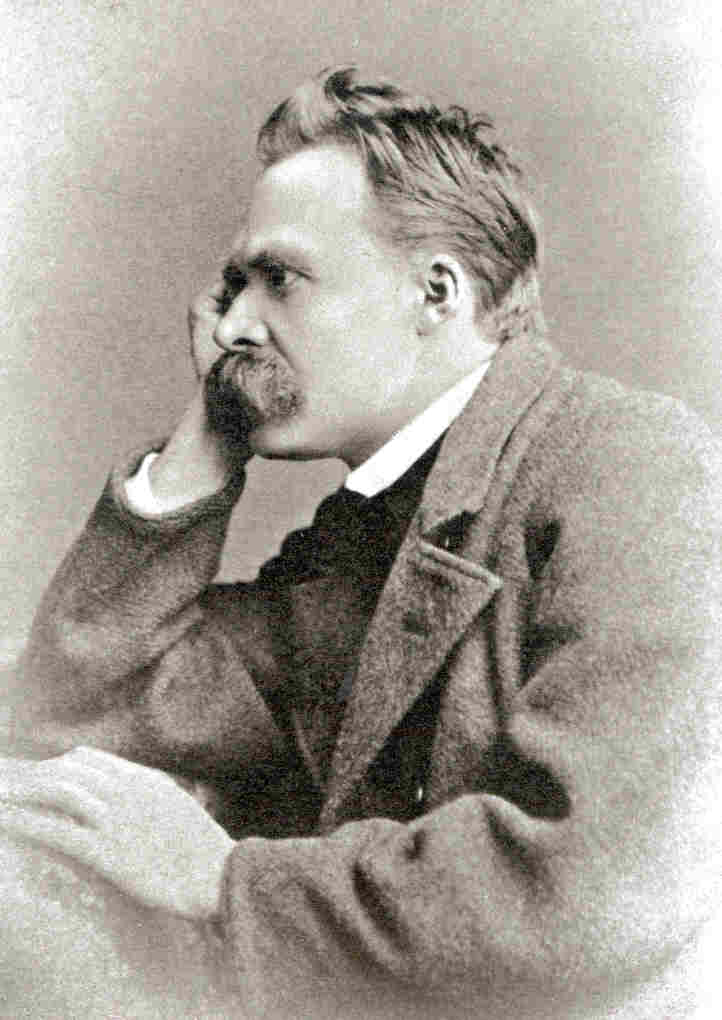
\includegraphics[height=4cm]{../../graphics/nietzsche.jpg}
            \end{column}
            \begin{column}{7cm}
                Insofar as moralized asceticism denies this worldly goods and pleasures in favor of the goods and pleasures of a fictitious other world it is fundamentally opposed to life. But as the priest and his morality are parts of life, then we have an apparent paradox: \alert{The ascetic priest is opposing life against life}.
            \end{column}
        \end{columns}
\end{frame}

\begin{frame}<presentation>[label=slide2]
    \frametitle{The Great Nausea at Man}
        \begin{columns}
            \begin{column}{3cm}
                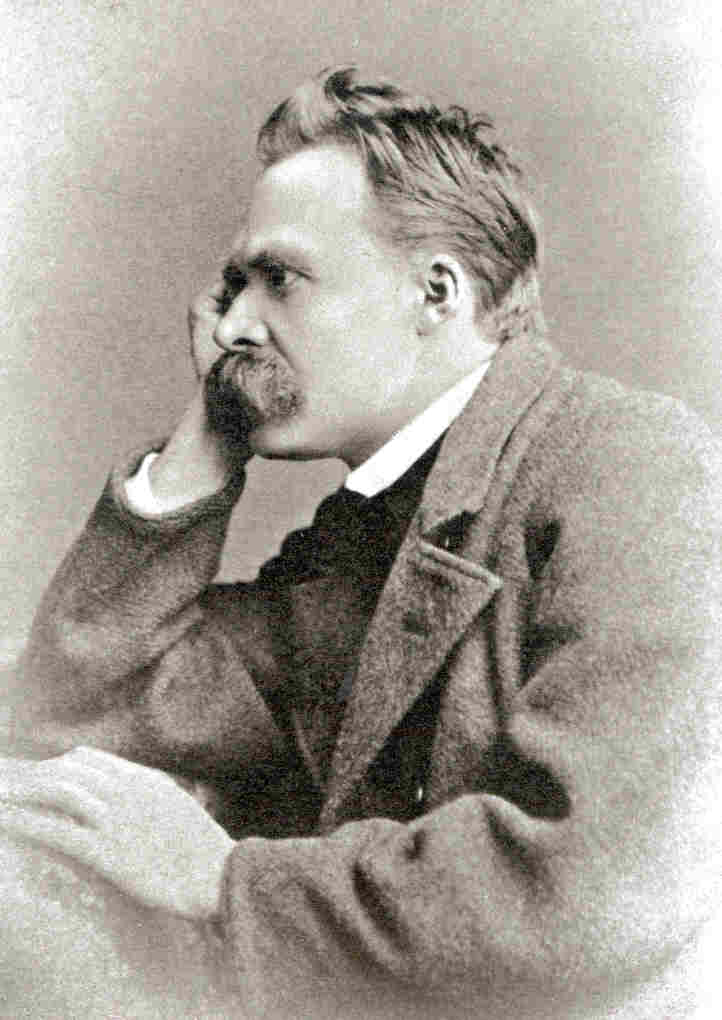
\includegraphics[height=4cm]{../../graphics/nietzsche.jpg}
            \end{column}
            \begin{column}{7cm}
                
            \end{column}
        \end{columns}
\end{frame}

\section*{Summary}

\end{document}
